% Options for packages loaded elsewhere
\PassOptionsToPackage{unicode}{hyperref}
\PassOptionsToPackage{hyphens}{url}
\PassOptionsToPackage{dvipsnames,svgnames,x11names}{xcolor}
%
\documentclass[
]{agujournal2019}

\usepackage{amsmath,amssymb}
\usepackage{iftex}
\ifPDFTeX
  \usepackage[T1]{fontenc}
  \usepackage[utf8]{inputenc}
  \usepackage{textcomp} % provide euro and other symbols
\else % if luatex or xetex
  \usepackage{unicode-math}
  \defaultfontfeatures{Scale=MatchLowercase}
  \defaultfontfeatures[\rmfamily]{Ligatures=TeX,Scale=1}
\fi
\usepackage{lmodern}
\ifPDFTeX\else  
    % xetex/luatex font selection
\fi
% Use upquote if available, for straight quotes in verbatim environments
\IfFileExists{upquote.sty}{\usepackage{upquote}}{}
\IfFileExists{microtype.sty}{% use microtype if available
  \usepackage[]{microtype}
  \UseMicrotypeSet[protrusion]{basicmath} % disable protrusion for tt fonts
}{}
\makeatletter
\@ifundefined{KOMAClassName}{% if non-KOMA class
  \IfFileExists{parskip.sty}{%
    \usepackage{parskip}
  }{% else
    \setlength{\parindent}{0pt}
    \setlength{\parskip}{6pt plus 2pt minus 1pt}}
}{% if KOMA class
  \KOMAoptions{parskip=half}}
\makeatother
\usepackage{xcolor}
\setlength{\emergencystretch}{3em} % prevent overfull lines
\setcounter{secnumdepth}{5}
% Make \paragraph and \subparagraph free-standing
\ifx\paragraph\undefined\else
  \let\oldparagraph\paragraph
  \renewcommand{\paragraph}[1]{\oldparagraph{#1}\mbox{}}
\fi
\ifx\subparagraph\undefined\else
  \let\oldsubparagraph\subparagraph
  \renewcommand{\subparagraph}[1]{\oldsubparagraph{#1}\mbox{}}
\fi


\providecommand{\tightlist}{%
  \setlength{\itemsep}{0pt}\setlength{\parskip}{0pt}}\usepackage{longtable,booktabs,array}
\usepackage{calc} % for calculating minipage widths
% Correct order of tables after \paragraph or \subparagraph
\usepackage{etoolbox}
\makeatletter
\patchcmd\longtable{\par}{\if@noskipsec\mbox{}\fi\par}{}{}
\makeatother
% Allow footnotes in longtable head/foot
\IfFileExists{footnotehyper.sty}{\usepackage{footnotehyper}}{\usepackage{footnote}}
\makesavenoteenv{longtable}
\usepackage{graphicx}
\makeatletter
\def\maxwidth{\ifdim\Gin@nat@width>\linewidth\linewidth\else\Gin@nat@width\fi}
\def\maxheight{\ifdim\Gin@nat@height>\textheight\textheight\else\Gin@nat@height\fi}
\makeatother
% Scale images if necessary, so that they will not overflow the page
% margins by default, and it is still possible to overwrite the defaults
% using explicit options in \includegraphics[width, height, ...]{}
\setkeys{Gin}{width=\maxwidth,height=\maxheight,keepaspectratio}
% Set default figure placement to htbp
\makeatletter
\def\fps@figure{htbp}
\makeatother
% definitions for citeproc citations
\NewDocumentCommand\citeproctext{}{}
\NewDocumentCommand\citeproc{mm}{%
  \begingroup\def\citeproctext{#2}\cite{#1}\endgroup}
\makeatletter
 % allow citations to break across lines
 \let\@cite@ofmt\@firstofone
 % avoid brackets around text for \cite:
 \def\@biblabel#1{}
 \def\@cite#1#2{{#1\if@tempswa , #2\fi}}
\makeatother
\newlength{\cslhangindent}
\setlength{\cslhangindent}{1.5em}
\newlength{\csllabelwidth}
\setlength{\csllabelwidth}{3em}
\newenvironment{CSLReferences}[2] % #1 hanging-indent, #2 entry-spacing
 {\begin{list}{}{%
  \setlength{\itemindent}{0pt}
  \setlength{\leftmargin}{0pt}
  \setlength{\parsep}{0pt}
  % turn on hanging indent if param 1 is 1
  \ifodd #1
   \setlength{\leftmargin}{\cslhangindent}
   \setlength{\itemindent}{-1\cslhangindent}
  \fi
  % set entry spacing
  \setlength{\itemsep}{#2\baselineskip}}}
 {\end{list}}
\usepackage{calc}
\newcommand{\CSLBlock}[1]{\hfill\break\parbox[t]{\linewidth}{\strut\ignorespaces#1\strut}}
\newcommand{\CSLLeftMargin}[1]{\parbox[t]{\csllabelwidth}{\strut#1\strut}}
\newcommand{\CSLRightInline}[1]{\parbox[t]{\linewidth - \csllabelwidth}{\strut#1\strut}}
\newcommand{\CSLIndent}[1]{\hspace{\cslhangindent}#1}

\usepackage{url} %this package should fix any errors with URLs in refs.
\usepackage{lineno}
\usepackage[inline]{trackchanges} %for better track changes. finalnew option will compile document with changes incorporated.
\usepackage{soul}
\linenumbers
\makeatletter
\@ifpackageloaded{caption}{}{\usepackage{caption}}
\AtBeginDocument{%
\ifdefined\contentsname
  \renewcommand*\contentsname{Table of contents}
\else
  \newcommand\contentsname{Table of contents}
\fi
\ifdefined\listfigurename
  \renewcommand*\listfigurename{List of Figures}
\else
  \newcommand\listfigurename{List of Figures}
\fi
\ifdefined\listtablename
  \renewcommand*\listtablename{List of Tables}
\else
  \newcommand\listtablename{List of Tables}
\fi
\ifdefined\figurename
  \renewcommand*\figurename{Figure}
\else
  \newcommand\figurename{Figure}
\fi
\ifdefined\tablename
  \renewcommand*\tablename{Table}
\else
  \newcommand\tablename{Table}
\fi
}
\@ifpackageloaded{float}{}{\usepackage{float}}
\floatstyle{ruled}
\@ifundefined{c@chapter}{\newfloat{codelisting}{h}{lop}}{\newfloat{codelisting}{h}{lop}[chapter]}
\floatname{codelisting}{Listing}
\newcommand*\listoflistings{\listof{codelisting}{List of Listings}}
\makeatother
\makeatletter
\makeatother
\makeatletter
\@ifpackageloaded{caption}{}{\usepackage{caption}}
\@ifpackageloaded{subcaption}{}{\usepackage{subcaption}}
\makeatother
\ifLuaTeX
  \usepackage{selnolig}  % disable illegal ligatures
\fi
\usepackage{bookmark}

\IfFileExists{xurl.sty}{\usepackage{xurl}}{} % add URL line breaks if available
\urlstyle{same} % disable monospaced font for URLs
\hypersetup{
  pdftitle={Unlocking Smart Growth: The Effects of Proposed Transit-Oriented Development Laws on the Puget Sound Region},
  pdfauthor={Tiernan Martin; Alex Brennan},
  pdfkeywords={Transit-Oriented Development, Growth Management
Act, Central Puget Sound Region, Washington State 2024 Legislative
Session},
  colorlinks=true,
  linkcolor={blue},
  filecolor={Maroon},
  citecolor={Blue},
  urlcolor={Blue},
  pdfcreator={LaTeX via pandoc}}

\journalname{Futurewise}

\draftfalse

\begin{document}
\title{Unlocking Smart Growth: The Effects of Proposed Transit-Oriented
Development Laws on the Puget Sound Region}

\authors{Tiernan Martin\affil{1}, Alex Brennan\affil{1}}
\affiliation{1}{Futurewise, }
\correspondingauthor{Tiernan Martin}{tiernan@futurewise.org}


\begin{abstract}
During the 2024 legislative session in Washington State, members of the
House of Representatives introduced a bill aimed at promoting community
and transit-oriented housing development. This, House Bill 2160,
proposed mandating cities to allow developments of a specific scale
within certain distances from high-capacity transit stops. This study
evaluates the extent to which the proposed increases in development
capacity under this bill exceed current allowances. The findings
indicate a substantial increase in development potential for the
majority of areas within walking distance of transit stops.
Specifically, for land that is developable and zoned for lower
development capacity than what the bills propose, the average increase
in capacity is projected to be an additional 1.35 floor area ratio
(FAR).
\end{abstract}

\section*{Plain Language Summary}
In 2024, the Washington State Legislature considered two new laws aimed
at making it easier to build homes near public transit areas, like light
rail stations and bus rapid transit stops. These laws would require
cities to allow taller, denser buildings in these areas. Our study
looked at how much more development could happen under these new laws
compared to what's currently allowed. We found that, if these laws pass,
there would be a lot more room for building new homes and apartments
near transit stops.



\subsection*{About Futurewise}\label{about-futurewise}
\addcontentsline{toc}{subsection}{About Futurewise}

\href{https://futurewise.org/}{\begin{center}

\includegraphics[width=1.5625in,height=\textheight]{images/Futurewise Logo.png}
\end{center}
}

Futurewise is a nonprofit organization that works throughout Washington
State on the implementation of the Growth Management Act (GMA). We
partner with local communities to support land use policies that
encourage healthy, equitable and opportunity-rich communities, and that
protect our most valuable farmlands, forests and water resources. We
have members across the state including the central Puget Sound region.
For more information about our organization, visit our website at
\url{https://futurewise.org/}.

\subsection*{Acknowledgments}\label{acknowledgments}
\addcontentsline{toc}{subsection}{Acknowledgments}

The authors received no financial support for the research, authorship,
or publication of this article.

Thanks to Yonah Freemark from the Urban Institute for providing zoning
district data.(Urban Institute, 2023) Thanks to Lauren Engel, Carol
Naito, and Robin Koskey from the Puget Sound Regional Council for
sharing the agency's public transit data and analysis of Washington
State House Bill 2160 and Senate Bill 6024.(Puget Sound Regional
Council, 2024) Thanks to Noha Mahgoub from the Office of Governor Jay
Inslee for providing feedback and guidance.

\subsection{Introduction}\label{introduction}

\begin{figure}[H]

{\centering 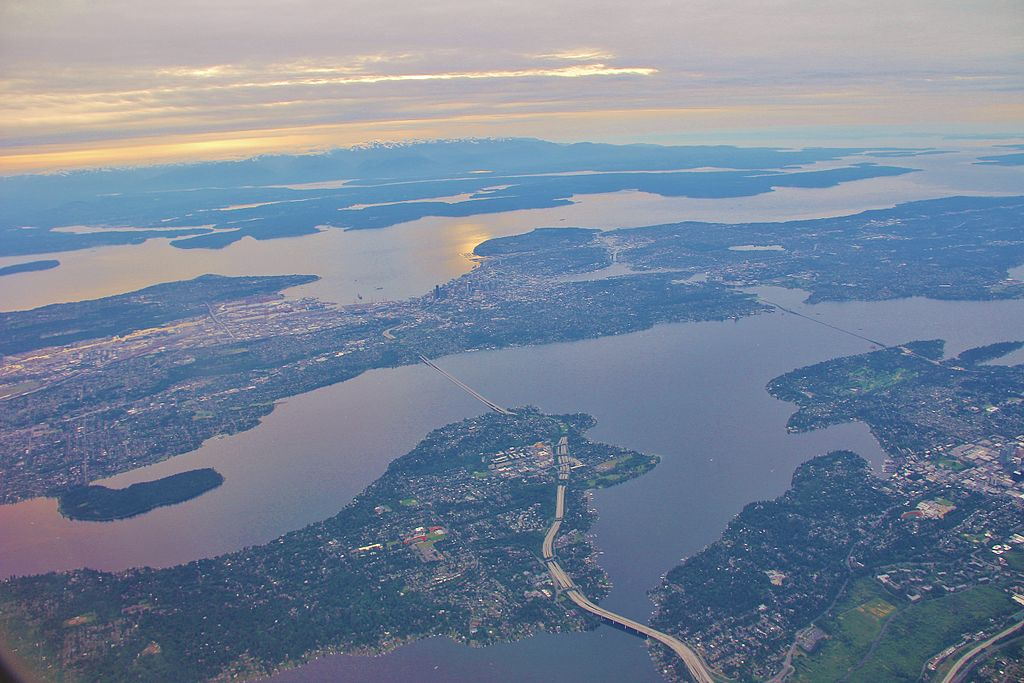
\includegraphics{images/seattle-aerial-wikicommons.jpg}

}

\caption{Central Puget Sound \textbar{} Photo courtesy of
\hyperref[0]{Clemens Vasters from Viersen, Germany}, \hyperref[0]{CC BY
2.0}, via Wikimedia Commons}

\end{figure}%

\subsubsection{The Central Puget Sound
Region}\label{the-central-puget-sound-region}

The Puget Sound metropolitan region is one of North America's major
growth centers for people, jobs, and housing. Between 2010 and 2023, the
central Puget Sound's four-county region (King, Snohomish, Pierce, and
Kitsap counties) added more residents and housing units than the rest of
Washington state combined.\footnote{The source of these statistics are
  the author's analysis of postcensial estimates by the Washington State
  Office of Financial Management. The central Puget Sound population
  grew by 414,400 people between 2010 and 2023, while the rest of the
  state's population grew by 84,300 people. During the same period,
  276,177 housing units were added in the this region, while 179,786
  units were created elsewhere in the state.} According to forecasts by
the Puget Sound Regional Council, the region's population is expected to
grow to 5.8 million people living within 2.8 million households by
2050.(Puget Sound Regional Council, 2018)

One challenge that the central Puget Sound region faces is high, rising
housing costs. The Puget Sound Regional Council's \emph{Housing
Stability Strategy: 2023 Monitoring Report} provides several sobering
statistics about the region's housing costs. According to the report,
during the decade between 2010 and 2020, the region added only one
housing unit for every three new people that were born or moved there.
By 2023, the annual income required to purchase the area's median priced
home was \$160,000.\footnote{This estimate includes three of the four
  central Puget Sound counties: King, Pierce, and Snohomish.} Between
July 2015 and July 2023, the median rent cost increased by 50\%.(Puget
Sound Regional Council, 2023a)

\subsubsection{Transit-Oriented
Development}\label{transit-oriented-development}

Transit-oriented development (TOD) is a strategy of building homes at or
near public transportation stops and stations. In the United States,
this strategy has had a complicated record---often leading to increased
property values while simultaneously lowering household travel costs and
reducing reliance on personal vehicles.(Lund, 2006) TOD often raises
concerns about the displacement of low-income residents and small
businesses, leading some local and regional governments to include
affordability requirements in their TOD programs.(Dawkins \& Moeckel,
2016)

While these concerns are valid, there is not an obvious, superior
alternative to TOD. Sharp increases in sprawling, low-density
residential and commercial development in Washington during 1980s
resulted in many unintended consequences, including ecological
disruption, traffic congestion, urban disinvestment, and loss of
agricultural lands.(Trohimovich, 2002) This led the Washington State
Legislature to adopt the Growth Management Act (GMA), a law requiring
cities and counties to plan to accommodate growth within designated
areas (urban growth areas or UGAs). Many of the GMA's planning goals are
highly aligned with TOD as a land use strategy---particularly the first
four goals of the law.\footnote{The first four goals of
  \href{https://app.leg.wa.gov/rcw/default.aspx?cite=36.70a.020}{\emph{RCW
  36.70A.020 Planning goals}} are:

  \begin{quote}
  (1) Urban growth. Encourage development in urban areas where adequate
  public facilities and services exist or can be provided in an
  efficient manner. (2) Reduce sprawl. Reduce the inappropriate
  conversion of undeveloped land into sprawling, low-density
  development. (3) Transportation. Encourage efficient multimodal
  transportation systems that will reduce greenhouse gas emissions and
  per capita vehicle miles traveled, and are based on regional
  priorities and coordinated with county and city comprehensive plans.
  (4) Housing. Plan for and accommodate housing affordable to all
  economic segments of the population of this state, promote a variety
  of residential densities and housing types, and encourage preservation
  of existing housing stock.
  \end{quote}}

\subsubsection{House Bill 2160}\label{house-bill-2160}

House Bill 2160 (HB 2160) of the 2023-2024 Washington State Legislative
Session proposed changes to the GMA intended to promote community and
transit-oriented housing development.\footnote{This study uses the
  Second Substitute of House Bill 2160 as the basis for its analysis.}
These changes, which would apply to all cities planning under the GMA,
included the following:

\begin{itemize}
\item
  Prohibiting cities from preventing the siting of multifamily housing
  on residential land within transit station areas
\item
  Prohibiting cities from enacting maximum floor area ratio (FAR)
  regulation under the following thresholds: 3.5 FAR for station areas
  of light rail, commuter rail, or streetcars; 2.5 FAR for station areas
  of bus rapid transit
\item
  Limits the ability of cities to require off-street parking of new
  residential or mixed-use projects
\item
  Categorically exempting residential or mixed-use projects within
  station areas from the State Environmental Policy Act (SEPA)
\end{itemize}

The bill also proposed several requirements of residential development
built within station areas, including making at least 10\% of its
residential units affordable.\footnote{The bill defines ``Affordable
  housing'' as:

  \begin{quote}
  {[}R{]}esidential housing whose monthly costs, including utilities
  other than telephone, do not exceed 30 percent of the monthly income
  of a household whose income is: (a) For rental housing, 60 percent of
  the median household income-adjusted for household size, for the
  county where the household is located, as reported by the United
  States department of housing and 5urban development; or (b) For
  owner-occupied housing, 80 percent of the median household income
  adjusted for household size, for the county where 8the household is
  located, as reported by the United States department of housing and
  urban development. (Reed, 2024)
  \end{quote}}

\subsubsection{Research Objective \&
Questions}\label{research-objective-questions}

The purpose of this study is to provide information about the effects of
the proposed HB 2160. Specifically, we seek to answer the following
questions:

\begin{enumerate}
\def\labelenumi{\arabic{enumi}.}
\item
  What are the characteristics of the current land uses of the transit
  station areas as defined in the bill?
\item
  Would this bill have an effect on the allowed development capacity of
  transit station areas?
\item
  What is the size of any effect this bill may have?
\item
  How are the bill's effects distributed between the two station area
  types that it defines?
\item
  What patterns are present in the cities that would be significantly
  impacted by the bill?
\end{enumerate}

\subsection{Data \& Methods}\label{sec-data-methods}

\subsubsection{Research Design}\label{research-design}

We use a quantitative method to attempt to answer our research
questions.

To quantify the impact of zoning changes on development capacity within
transit areas, we define the area-weighted mean of net development
capacity (\(AWM_{NDC}\)) as follows:

\[
AWM_{NDC} = \frac{\sum_{i}(NDC_i \cdot A_i \cdot I_i)}{\sum_{i}(A_i \cdot I_i)}
\]

where:

\begin{itemize}
\tightlist
\item
  \(NDC_i = FAR_{new,i} - FAR_{old,i}\) represents the net development
  capacity for parcel \(i\), calculated as the difference between the
  new Floor Area Ratio (FAR) and the old FAR. Where \(NDC_i < 0\), we
  set it equal to 0 because the bill would not reduce maximum FAR.
\item
  \(A_i\) denotes the area of parcel \(i\).
\item
  \(I_i\) is an indicator function that equals 1 if parcel \(i\)
  satisfies all of the following conditions: it is within a station
  area, it lies within a zoning district where residential use is
  permitted, and it is within an urban growth area; otherwise, \(I_i\)
  equals 0.
\end{itemize}

This formula ensures that the calculation exclusively incorporates
parcels meeting the specified criteria, with each parcel's contribution
to the overall mean being proportionally weighted by its area.

Our method offers a precise metric for evaluating changes in development
capacity, reflecting the effects of the proposed bill. It also allows us
to summarize the bills effect at different geographic levels, including
station area, city, and region. We can then both describe individual
geographies (e.g., a specific station area) and compare between
geographies (e.g., several cities compared individually to the region).

\subsubsection{Data Collection}\label{data-collection}

The study uses several data sets from a variety of different sources.
The following table summarize the study's data:

\begin{longtable}[]{@{}
  >{\raggedright\arraybackslash}p{(\columnwidth - 4\tabcolsep) * \real{0.3333}}
  >{\raggedright\arraybackslash}p{(\columnwidth - 4\tabcolsep) * \real{0.3333}}
  >{\raggedright\arraybackslash}p{(\columnwidth - 4\tabcolsep) * \real{0.3333}}@{}}
\toprule\noalign{}
\begin{minipage}[b]{\linewidth}\raggedright
Data
\end{minipage} & \begin{minipage}[b]{\linewidth}\raggedright
Description
\end{minipage} & \begin{minipage}[b]{\linewidth}\raggedright
Citation
\end{minipage} \\
\midrule\noalign{}
\endhead
\bottomrule\noalign{}
\endlastfoot
Current Parcels (2023) & A statewide data set of tax parcels &
Washington State Parcels Project (2023) \\
Transit Stations & Transit station locations for light rail, commuter
rail, streetcar, and existing bus rapid transit routes in the central
Puget Sound Region & Puget Sound Regional Council (2024) \\
Puget Sound Zoning Districts (2023) & Zoning and land use regulations
collected from central Puget Sound local governments' land use codes and
maps & Urban Institute (2023) \\
Urban Growth Areas & Urban growth areas for the central Puget Sound
region (King, Snohomish, Kitsap, and Pierce counties) & Puget Sound
Regional Council (2023b) \\
\end{longtable}

\subsubsection{Data Analysis}\label{data-analysis}

The study uses a combination of a relational database and statistical
software to conduct its analysis. The relational database, PostgreSQL
with the PostGIS extension, is used to perform spatial filters and
spatial joins on the Current Parcel data set. The R programming language
is used to perform aggregations and calculate summary statistics on the
filtered and augmented parcel dataset. R is also also used to produce
summary tables and visualizations.

Data sets containing information relevant to HB 2160 are combined
through spatial filtering and spatial joining to produce a data set of
all parcels within the station areas. The refined parcel data are
augmented with zoning and land use regulation information from the
zoning districts. A maximum FAR baseline is estimated for all parcels,
then the new maximum FAR that would be introduced by HB 2160 is
estimated. For each parcel, the net difference between the current (old)
and new FAR is calculated. For parcels where the current zoning allows
development greater than the new FAR, the effect of the bill is
considered to be zero additional FAR; for parcels where the current
zoning is more restrictive that the new FAR, the effect is calculated in
terms of additional FAR allowed. The bill's effect on each parcel is
then aggregated by station area, jurisdiction, and region, and
summarized using the area-weight mean.\footnote{Parcels that do not
  allow residential uses are characterized as ``not developable'' and
  are not included in the area-weighted mean statistic; however, these
  parcels are included in the study's analysis for other purposes such
  as describing and quantithe characteristics of land within each
  station area or jurisdiction.}

\subsubsection{Limitations}\label{limitations}

Our method is subject to several limitations that are important to
consider when interpreting our findings:

\begin{enumerate}
\def\labelenumi{\arabic{enumi}.}
\item
  \textbf{Scope of Parcels}: The study is limited to parcels where
  residential use is permitted. This exclusion may omit significant
  areas that could be relevant under different zoning changes or future
  development scenarios.
\item
  \textbf{Measurement of Transit Proximity}: Transit walksheds are
  calculated using Euclidean distance, measuring straight lines to the
  center of parcels, rather than using network distances that reflect
  actual walking paths. This method may overestimate or underestimate
  the true accessibility of parcels to transit services.
\item
  \textbf{Lot Coverage Assumptions}: In cases where specific regulations
  on maximum building footprint or FAR are not provided, the study
  assumes that 100\% lot coverage is permissible. This assumption may
  not align with actual zoning regulations, potentially leading to
  overestimations of development capacity.
\item
  \textbf{Omission of Development Regulations}: The estimated FAR metric
  does not incorporate other development regulations, such as setbacks,
  which can significantly impact the buildable area on a parcel.
\item
  \textbf{Homeowner Association (HOA) Restrictions}: The analysis does
  not consider HOA restrictions that might limit allowed density on
  parcels, which could reduce the impact of bill in station areas where
  restrictive HOA's exist.
\item
  \textbf{Housing Unit Limits Ignored}: The study does not account for
  maximum unit limits that can further restrict the number of residences
  within a given development, possibly leading to inaccurate assessments
  of potential housing contributions.
\item
  \textbf{Regulatory Combinations Not Considered}: Interactions between
  different regulations, such as maximum building height and maximum
  FAR, are not accounted for. This omission can lead to an
  oversimplification of the practical limits on parcel development.
\item
  \textbf{Additional Restrictions on Development}: The analysis does not
  account for other significant restrictions, including those that
  prevent development from being sited within critical areas, shoreline
  environments, or on sites with landmark designations. Such
  restrictions can materially impact development possibilities but are
  not reflected in the study.
\item
  \textbf{Currency of Data}: The study assumes that all data used in the
  analysis are concurrent and up-to-date. Any discrepancies in data
  timeliness could affect the accuracy of the results.
\end{enumerate}

Further research, data collection, and methodological refinements could
help address these limitations in future analyses.

\subsection{Results}\label{results}

The study included approximately 125,000 parcels (\(N = 124,941\)), all
within the four central Puget Sound counties, within an Urban Growth
Area, and within HB 2160's specified distance thresholds of a qualifying
transit stop.

We separated the study data into three analysis groups:

\begin{enumerate}
\def\labelenumi{\arabic{enumi}.}
\item
  \textbf{Not Developable}\\
  Parcels that do not meet the study's eligibility criteria. These
  criteria include allowing residential uses and having a tax
  assessor-assigned land use that is compatible with
  development.\footnote{For the purposes of this study, tax
    assessor-assigned land uses that are \emph{not compatible} with
    development are: `Non commercial forest', `Open space land
    classified under chapter 84.34 RCW', and `Water areas'.}
\item
  \textbf{Developable, Not Affected}\\
  Parcels that meet the study's eligibility criteria but have an equal
  or higher development capacity than the bill would allow and would,
  therefore, not be affected by the bill.
\item
  \textbf{Developable, Affected}\\
  Parcels that meet the study's eligibility criteria and have zoning
  that is more restrictive than the maximum FAR set by the bill and
  would, therefore, be affected.
\end{enumerate}

\begin{longtable}[]{@{}lrr@{}}
\caption{Study Summary Statistics: Central Puget Sound}\tabularnewline
\toprule\noalign{}
Analysis Group & Parcels (N) & Land Area (sq. miles) \\
\midrule\noalign{}
\endfirsthead
\toprule\noalign{}
Analysis Group & Parcels (N) & Land Area (sq. miles) \\
\midrule\noalign{}
\endhead
\bottomrule\noalign{}
\endlastfoot
Not Developable & 7,219 & 16.80 \\
Developable, Not Affected & 20,288 & 23.48 \\
Developable, Affected & 97,434 & 72.77 \\
Total & 124,941 & 113.04 \\
\end{longtable}

\textsubscript{Source:
\href{https://tiernanmartin.github.io/2024-transit-oriented-development-bill/index-preview.html}{Article
Notebook}}

We find that approximately most parcels and most land area within the
station areas would be affected by the bill:

\begin{longtable}[]{@{}lll@{}}
\caption{Study Summary Statistics: Affected Parcels, Central Puget
Sound}\tabularnewline
\toprule\noalign{}
Analysis Group & Parcels (\%) & Land Area (\%) \\
\midrule\noalign{}
\endfirsthead
\toprule\noalign{}
Analysis Group & Parcels (\%) & Land Area (\%) \\
\midrule\noalign{}
\endhead
\bottomrule\noalign{}
\endlastfoot
Developable, Affected & 78\% & 64\% \\
\end{longtable}

\textsubscript{Source:
\href{https://tiernanmartin.github.io/2024-transit-oriented-development-bill/index-preview.html}{Article
Notebook}}

\begin{figure}[H]

{\centering 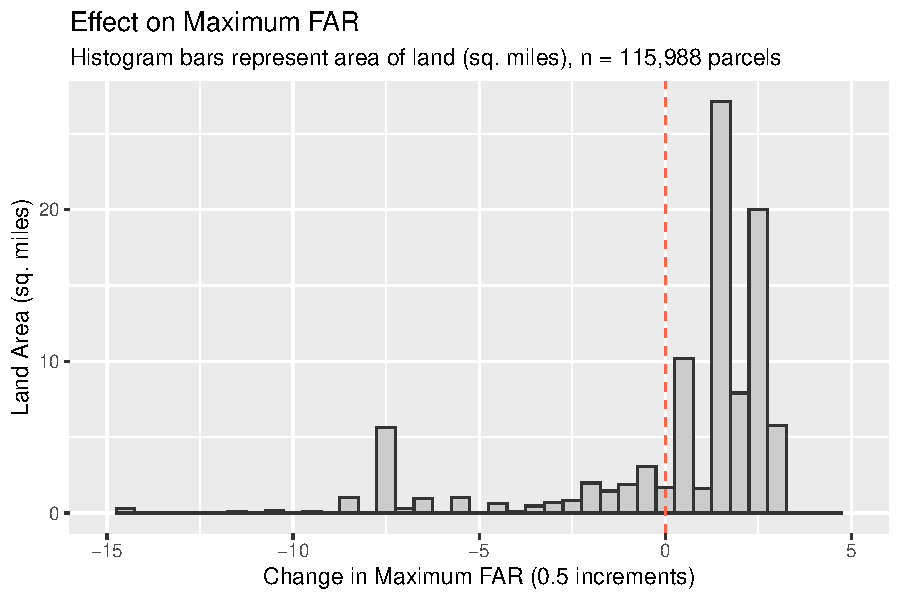
\includegraphics{index_files/figure-pdf/results-histogram-1.pdf}

}

\caption{HB 2160s Effect on Maximum FAR}

\end{figure}%

\textsubscript{Source:
\href{https://tiernanmartin.github.io/2024-transit-oriented-development-bill/index-preview.html}{Article
Notebook}}

\subsection{Discussion}\label{discussion}

\subsection{Conclusion}\label{conclusion}

\subsection*{References}\label{references}
\addcontentsline{toc}{subsection}{References}

\phantomsection\label{refs}
\begin{CSLReferences}{1}{0}
\vspace{1em}

\bibitem[\citeproctext]{ref-dawkins2016}
Dawkins, C. J., \& Moeckel, R. (2016). Transit-induced gentrification:
Who will stay, and who will go? \emph{Housing Policy Debate}, \emph{26},
801--818. \url{https://doi.org/10.1080/10511482.2016.1138986}

\bibitem[\citeproctext]{ref-lund2006}
Lund, H. (2006). Reasons for living in a transit-oriented development,
and associated transit use. \emph{Journal of the American Planning
Association}, \emph{72}, 357--366.
\url{https://doi.org/10.1080/01944360608976757}

\bibitem[\citeproctext]{ref-pugetsoundregionalcouncil2018}
Puget Sound Regional Council. (2018). \emph{Draft 2050 forecast of
people and jobs}. Retrieved from \url{https://www.psrc.org/media/1749}

\bibitem[\citeproctext]{ref-pugetsoundregionalcouncil2023}
Puget Sound Regional Council. (2023a). \emph{Regional housing strategy:
2023 monitoring report}. Retrieved from
\url{https://www.psrc.org/sites/default/files/2023-11/reg-housing-strategy-monitoring-rpt-2023.pdf}

\bibitem[\citeproctext]{ref-pugetsoundregionalcouncil}
Puget Sound Regional Council. (2023b, September). PSRC data portal.

\bibitem[\citeproctext]{ref-pugetsoundregionalcouncil2024}
Puget Sound Regional Council. (2024, January). Community and
transit-oriented housing development bill 2024: An interactive web map.
Retrieved from \url{https://arcg.is/0SSvK10}

\bibitem[\citeproctext]{ref-reed2024}
Reed, R. J. (2024). An act relating to promoting community and
transit-oriented housing development.

\bibitem[\citeproctext]{ref-trohimovich2002}
Trohimovich, T. (2002). The growth management act (GMA) after more than
10 years: Another look \& a response to criticisms. \emph{Growth}.
Retrieved from
\url{http://www.futurewise.org/assets/resources/GMA_another_look.pdf}

\bibitem[\citeproctext]{ref-urbaninstitute}
Urban Institute. (2023). Urban institute puget sound zoning atlas.

\bibitem[\citeproctext]{ref-washingtonstateparcelsproject}
Washington State Parcels Project. (2023). Current parcels (2023).

\end{CSLReferences}



\end{document}
